\newcommand{\nl}{$n_{\ell}$ }
\newcommand{\km}{\textless k \textgreater}
\chapter{Structure des réseaux sans-échelle non corrélés: couches et plus court chemin}
\label{sec3}
L'objectif principal de ce chapitre vise à prédire quel sera le comportement des systèmes en réseau sur la base des propriétés structurelles mesurées et des règles locales régissant les sommets individuels. Comment, par exemple, la distribution des degrés du réseau affectera-t-elle sa  structure et ses propriétés ?

\section{Introduction}

De nombreux réseaux du monde réel qui ont été décrits précédemment, tels que le WWW et les réseaux de collaboration, grandissent avec le temps. Par conséquent, il est raisonnable de considérer les graphes de taille croissante et d'étudier la structure de ces réseaux ayant souvent la propriété sans-échelle (voir Section.\ref{s-libre-echelle}). 
La communauté scientifique, en s'appuyant sur des idées issues d'une grande variété de disciplines, a fait un excellent départ sur la caractérisation et la modélisation de la structure des réseaux, mais il n 'y pas encore des progressions théoriques cruciaux dans ce domaine \cite{Ne2003}. Ici nous allons considérer ces problèmes en donnant quelques contributions à ces études concernant la structure des réseaux sans-échelle, et en trouvant pour la première fois les expressions explicites des couches, ainsi que, des formules plus précises du plus court chemin par rapport aux anciens résultats existant dans la littérature. 
\section{Les réseaux sans-échelle non corrélés}
Dans les modèles aléatoires sans-échelle, on suppose généralement qu'il n'y a pas de corrélation entre les degrés des nœuds voisins. C'est-à-dire que la probabilité d'atteindre un nœud en suivant un lien est indépendante du nœud d'où provient le lien. Cependant, dans de nombreux réseaux du monde réel, ce n'est pas le cas. Plusieurs types de corrélation existent, en fonction des propriétés internes des nœuds, les principaux types de corrélations étudiés sont les corrélations degré-degré (voir Section.\ref{s-correl}). Même si la construction de ces réseaux sans-échelle aléatoires se fait au début sans aucune corrélation, cela ne signifie pas que le réseau n'affichera pas des corrélations de degré, c'est-à-dire l'absence des corrélation lors de création des réseaux n'est pas une condition cruciale de l'absence de corrélation dans le réseau final, par exemple la Fig.~\ref{correlation} indique que les réseaux aléatoires sans-échelle génèrent des corrélations de degré, allant de l'assortativité à la disassortativité selon la valeur de l'exposant $\gamma$\footnote{$\gamma$ représente l'exposant de la distribution des degrés, $P(k)\propto k^{-\gamma}$, dans les réseaux sans-échelle }, nous observons trois régimes d'échelle distincts:
%\begin{spacing}{1.5}
\begin{itemize}
	\item[i)] Régime assortatif: $\gamma>3$
	\item[ii)]Régime neutre: $\gamma=3$
	\item[iii)] Régime disassortatif: $\gamma<3$
\end{itemize}
%\end{spacing}

Produire des corrélations en utilisant un modèle complètement statique est difficile car non seulement le degré d'un nœud doit être pris en compte, mais aussi sa probabilité de se connecter à chaque voisin. La méthode habituellement utilisée pour générer de tels réseaux consiste à mélanger les liens en utilisant une sorte d'algorithme de type Metropolis\footnote{Inventé en 1953 par Nicholas Metropolis et ses collaborateurs du laboratoire de Los Alamos, l'algorithme de Metropolis était d'abord destiné à faire calculer par des ordinateurs les équations d'états de mélanges de molécules en interactions. Depuis lors il s'est révélé bien adapté pour résoudre de nombreux problèmes de mécanique statistique et de chimie. L'outil principal de l'algorithme est une chaîne de Markov : on tire au hasard une boule et on déplace son centre d'une distance $d$, le mouvement est accepté si la nouvelle configuration des boules reste sans recouvrement.} \cite{Metropolis-al1953}.\\ Cependant, la négligence de ces corrélations n'empêche jamais de trouver des résultats importants qui nous aideront à bien modéliser ces réseaux réels et à mieux comprendre leurs structures. 
\begin{figure}[h!]
	\centering
	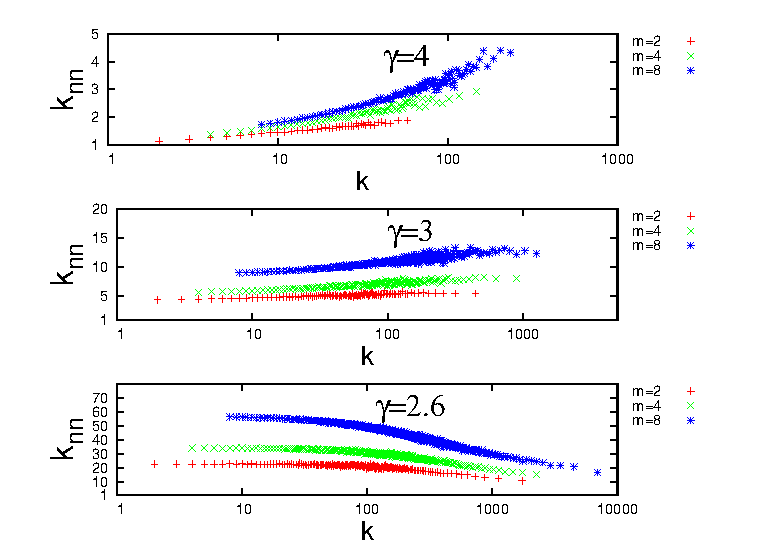
\includegraphics[scale=1.2]{./figures/correlation}
	\caption{Les corrélations des degrés dans le réseau aléatoire sans-échelle pour différentes valeurs de $m$ et de $\gamma$. Le nombre de nœuds est $n=10^4$ et le nombre de réalisations pour chaque simulations est $50$.}
	\label{correlation}
\end{figure}
\vspace{3cm}


\section{Les anciennes études sur les couches et le plus court chemin}
\subsection{Les couches}
Newman \cite{Newman2010-456} a calculé l'expression des couches, c'est-à-dire le nombre moyen de nœuds, \nl, à distance $\ell$ depuis un nœud arbitraire pour un réseau aléatoire, et il a donné l'expression: ~\nl$=\Big(\frac{n_2}{n_1}\Big)^{\ell-1}n_1$, où $n_1$ et $n_2$ sont le nombre moyen du premier et second voisins. Cela signifie que \nl augmente ou diminue avec $\ell$ selon que $n_2$ est supérieur ou inférieur à $n_1$. Cohen et al \cite{Cohen-Havlinl2010-72,Kalisky-al2006} ont considéré un réseau sans échelle spécifique et ont étudié les couches entourant le nœud le plus connecté, ils ont obtenu une relation de récurrence pour \nl. Ces calculs semblent bien cadrer avec les données Internet réelles dans le cas particulier de $m=1$, où $m$ est le degré minimum dans le réseau. Deux régimes sont observés pour \nl: le premier est caractérisé par une croissance rapide, et le second descend de façon exponentielle.\\
Ces deux études ne sont pas satisfaisantes, car la première expression de Newman est une fonction monotone, soit croissante ou décroissante, ce qui est conceptuellement faux \cite{Cohen-Havlinl2010}, et dans le deuxième résultat, Cohen et al.  n'ont pas réussi à trouver une expression explicite, mais plutôt une suite de récurrences sans solution.En plus leurs expressions correspondent plus aux données d'Internet et ne représentent aucune généralité.
 
\subsection{Plus court chemin}
\label{PCC}
 Le plus court chemin (PCC) peut être le concept le plus intrigant dans les réseaux complexes et la théorie des graphes, principalement après la célèbre expérience de Milgram \cite{Mi1967}. Dans cette expérience, Milgram a clairement démontré le phénomène du petit monde dans les réseaux sociaux, ce qui signifie que deux personnes dans le monde sont en moyen séparées par des petites connexions intermédiaires.\\
 Nous pouvons citer les anciennes formules du PCC  en relation avec la valeur de l'exposant $\gamma$ comme ceci : Pour $2<\gamma<3$ on dit que le réseau est ultra-petit $\textless\ell\textgreater\sim \ln\ln(n)$ \cite{Cohen-Havlin2003,Do-al2003,Cohen-al2002,Chung-Lu2002,Fox-Bellwood2014,Hofstad-al2014}, pour $\gamma=3$ on dit que le réseau est petit-monde $\textless\ell\textgreater\sim\frac{\ln(n)}{\ln\ln(n)}$ \cite{Bollobas1985,Chung-Lu2002,Fronczak-al2004,Hofstad-al2004,Cohen-Havlin2009} et pour $\gamma>3$ le réseau est aussi petit-monde $\textless\ell\textgreater\sim\ln(n)$ \cite{Bollobas1985,Chung-Lu2002,Fronczak-al2004,Hofstad-al2004,Cohen-Havlin2009}.  

\section{Structure des couches dans les réseaux sans-échelle non corrélés}
        \subsection{L'étude théorique}
La couche dans un réseau complexe est définie comme l'ensemble des nœuds à la même distance d'un nœud arbitraire choisi. Dans un réseau sans-échelle, chaque nœud est lié à d'autres nœuds $k$ avec la probabilité $P(k)=Ck^{-\gamma}$, $k=m, m + 1, \ldots, K$. Où $C=(\gamma-1)m^{\gamma-1}$ est la constante de normalisation, $m$ et $K$ sont les seuils inférieur et supérieur de la distribution. $K=mn^{\frac{1}{\gamma-1}}$, avec $n$ est le nombre total de nœuds. \\
Nous construisons un réseau sans-échelle en choisissant aléatoirement un nœud de degré moyen $\km$, et dans chaque couche suivante, nous mettons le degré suivant le plus élevé jusqu'à ce que la couche soit pleine (Fig.~\ref{fig1}).\\
\begin{figure}[h]
	\centering
	\begin{tikzpicture}[scale=0.25]
	\tikzstyle{lien}=[-,thick,circle]
	\tikzset{individu/.style={draw,circle,scale=1.8,fill=black},individu/.default={green},scale=0.65}
	\node[individu,scale=0.3] (a0) at (-1,0) {};
	\node[individu,scale=0.6] (a1) at (2.5,-8) {};
	\node[individu,scale=0.52] (a2) at (-1,-9.18) {};
	\node[individu,scale=0.46] (a3) at (-4.5,-8) {};
	\node[individu,scale=0.44] (b1) at (5,-15.5) {};
	\node[individu,scale=0.42] (b2) at (3,-16.55) {};
	\node[individu,scale=0.4] (b3) at (1.,-17.25) {};
	\node[individu,scale=0.38] (b4) at (-1,-17.6) {};
	\node[individu,scale=0.36] (b5) at (-3.,-17.45) {};
	\node[individu,scale=0.34] (b6) at (-5,-16.92) {};
	\node[individu,scale=0.32] (b7) at (-7,-16.1) {};
	\node[individu,scale=0.3] (c1) at (8,-23.7) {};
	\node[individu,scale=0.28] (c2) at (5.2,-25.1) {};
	\node[individu,scale=0.26] (c3) at (3.,-25.9) {};
	\node[individu,scale=0.24] (c4) at (1,-26.28) {};
	\node[individu,scale=0.22] (c5) at (-1,-26.4) {};
	\node[individu,scale=0.2] (c6) at (-3,-26.3) {};
	\node[individu,scale=0.18] (c7) at (-5,-26.3) {};
	\node[individu,scale=0.16] (c8) at (-7,-26.1) {};
	\node[individu,scale=0.14] (c9) at (-9,-25.30) {};
	\node[individu,scale=0.12] (c10) at (-11,-24.10) {};
	\node[individu,scale=0.10] (c11) at (-13,-23.21) {};
	\draw[-,>=latex,dashed] (c11) to[bend right] (c1);
	\draw[-,>=latex,dashed] (b7) to[bend right] (b1);
	\draw[-,>=latex,dashed] (a3) to[bend right] (a1);
	\draw[lien] (a0) -- (a1);
	\draw[lien] (a0) -- (a2);
	\draw[lien] (a0) -- (a3);
	\draw[lien] (a1) -- (b1);
	%\draw[lien] (a1) -- (b2);
	%\draw[lien] (a1) -- (b3);
	\draw[lien] (a1) -- (b5);
	\draw[lien] (a1) -- (b4);
	\draw[lien] (a2) -- (b6);
	\draw[lien] (a2) -- (b2);
	%\draw[lien] (a2) -- (b6);
	\draw[lien] (a3) -- (b3);
	\draw[lien] (a3) -- (b7);
	\draw[lien] (b1) -- (c1);
	\draw[lien] (b1) -- (c2);
	%\draw[lien] (b1) -- (c4);
	\draw[lien] (b1) -- (c5);
	%\draw[lien] (b2) -- (c1);
	\draw[lien] (b2) -- (c4);
	\draw[lien] (b3) -- (c3);
	\draw[lien] (b4) -- (c7);
	\draw[lien] (b3) -- (c8);
	\draw[lien] (b2) -- (c6);
	\draw[lien] (b5) -- (c10);
	\draw[lien] (b6) -- (c9);
	%\draw[lien] (b7) -- (c7);
	\draw[lien] (b7) -- (c11);
	\draw (-21,-7.5) node[right]{$l_1$,$n_1=\textless k \textgreater$};
	\draw (-15,-15.7) node[right]{$l_2$,$n_2$};
	\draw (-19.,-23) node[right]{$l_3$,$n_3$};
	\draw (3.3,-8) node[right]{$K_1=K$};
	\draw (5.4,-15.5) node[right]{$K_2$};
	\draw (8.1,-23.7) node[right]{$K_3$};
	\end{tikzpicture}
	\caption{Illustration du réseau construit. La taille des cercles pleins (nœuds) est le degré dépendant. Le degré maximum de couche $\ell$ est $K_{\ell}$.\\}
	\label{fig1}
\end{figure}

Évidemment, la première couche contiendra les premiers voisins $\km$ du nœud de départ, alors $n_1=\km$. Cela ne représente pas un réseau particulier, mais c'est juste une description idéalisée de tout réseau sans échelle. \\
Pour les grands réseaux non corrélés, la structure arborescente peut être supposée et les cycles dans la même couche sont négligés \cite{Cohen-Havlin2003,Cohen-Havlin2009}. Par la suite, la probabilité $ p_{\ell} $ qu'un nœud de la couche $n_\ell$ soit lié à un autre nœud n'appartenant pas aux premiers $\ell$ couches est $p_{\ell}=\frac{\kappa_{\ell}-1}{n}$, où $\kappa_{\ell}$ est le degré moyen des nœuds appartenant à la couche $n_\ell$ et le $-1$ est dû au lien de la couche précédente. \\
La probabilité que des nœuds parmi $n-n_1-1$ ne soient lié à aucun nœud dans $\ell=1$ est $(1-p_1)^{n_1}$, alors la probabilité que ces nœuds soient liés aux nœuds dans $\ell=1$ est $1-(1-p_1)^{n_1}$. Le nombre de nœuds dans $\ell=2$ est alors donné par $n_2=(1- (1-p_1)^{n_1})(n-n_1-1)$. La généralisation pour \nl est simple, on obtient:
\begin{align}
n_{\ell}= (1-(1-p_{\ell-1})^{n_{\ell-1}})(n-\sum_{j=1}^{\ell-1} n_j-1),
\label{eq1}
\end{align}
lorsque $n$ est grand $p_{\ell}\ll1 \Longrightarrow (1-p_{\ell-1})^{n_{\ell-1}}\simeq e^{-p_{\ell-1}n_{\ell-1}} $. Eq.~\eqref{eq1}
peut être facilement manipulé pour obtenir:
\begin{align}
n_{\ell} &=
\begin{cases}
\km & \text{si}\qquad \ell=1 \\
(n-1-n_1)(e^{-\sum_{j=1}^{\ell-2}p_j n_j}-e^{-\sum_{j=1}^{\ell-1}p_j n_j}) & \text{si}\qquad \ell \ge 2.
\end{cases}
\label{eq2}
\end{align}
L'équation ci-dessus peut être simplifiée en développant les sommes en exponentielles. $p_{\ell}$ est $\kappa_{\ell}$-dépendante, qui dépend à son tour de $\gamma$ et du degré maximal dans la couche $\ell$, $K_{\ell}$. D'abord on donne l'expression de $\kappa_{\ell}$ quand $K_{\ell}\gg m$, et ensuite on développe la somme sur $n_j$.
\begin{align}
\kappa_{\ell} =\frac{<k_{\ell}^2>}{\textless k_{\ell} \textgreater}=&
\begin{cases}
\Big(\frac{\gamma-2}{\gamma-3}\Big)m & \text{si} \qquad \gamma >3 \\ 
m (\log(K_{\ell})-\log(m))  & \text{si} \qquad \gamma =3 \\
\Big(\frac{\gamma-2}{3-\gamma}\Big)m^{\gamma-2} K_{\ell}^{3-\gamma}  & \text{si} \qquad 2<\gamma<3 \\
\frac{K_{\ell}-m}{\log(K_{\ell})-\log(m)} & \text{si} \qquad \gamma=2.
\end{cases}
\label{eq4}
\end{align}
Lorsque $\gamma=2$, le degré maximum $K_1$ est de l'ordre du nombre total de nœuds, c'est-à-dire que presque tous les nœuds sont connectés au nœud de degré maximal. Le réseau peut contenir un maximum de deux couches, avec $n_1=\km$ et $n_2=n-\km $. \\
Quand $2\textless \gamma \textless 3$, le réseau est encore très hétérogène. $\kappa_{\ell} $ est couche-dépendent, il dépend du degré maximal $K_{\ell} $ de la couche $\ell$ (Eq.~\eqref{eq4}). L'étape suivante de nos calculs consiste à relier $\kappa_{\ell}$ à $\kappa_1$. Le nombre de nœuds entre le premier et le $(\ell-1)^{\text{ème}}$ couches est donné par:
\begin{align}
\sum_{j=1}^{\ell-1}n_j&=n\int_{K_{\ell}}^{K_1} P(k)dk \nonumber \\
&=nm^{\gamma-1}(K_{\ell}^{1-\gamma}-K_1^{1-\gamma})\simeq nm^{\gamma-1} K_{\ell}^{1-\gamma},
\label{eq5}
\end{align}
où nous avons utilisé $K_1\gg K_{\ell}$ pour $n$ assez grand. Dans ce cas où $2\textless \gamma \textless 3$, $\kappa_{\ell}\gg 1$, alors
\begin{align}
\sum_{j=1}^{\ell-1}n_j&=\km+\km(\kappa_1-1)+\km(\kappa_1-1)(\kappa_2-1)+\ldots+\km(\kappa_1-1)(\kappa_2-1)\ldots(\kappa_{\ell-1}-2)\nonumber \\
&\approx\km\kappa_1\kappa_2\ldots\kappa_{\ell-2},
\label{eq6}
\end{align}
on en déduit
$K_{\ell}=\Big(\frac{\km\kappa_1\kappa_2\ldots\kappa_{\ell-2}}{nm^{\gamma-1}}\Big)^{\frac{1}{1-\gamma}}$.\\
Le degré moyen des voisins à distance $\ell $ peut maintenant être exprimé comme ceci :
$\kappa_{\ell}=\frac{\gamma-2}{3-\gamma}m\Big(\frac{n}{\km\kappa_1\kappa_2\ldots\kappa_{\ell-2}}\Big)^{\frac{3-\gamma}{\gamma-1}}$, ce qui conduit à la relation de récurrence $\kappa_{\ell}=\kappa_{\ell-1}
\Big(\kappa_{\ell-2}\Big)^{\frac{\gamma-3}{\gamma-1}}$.  Quand $\gamma$ est dans $]2,3[$ nous avons généralement
$\kappa_{\ell-2} \gg \kappa_{\ell-1}$  mais depuis $\mid\frac{\gamma-3}{\gamma-1}\mid<1$, on considère que $\Big(\kappa_{\ell-2}\Big)^{\frac{\gamma-3}{\gamma-1}}\approx
\Big(\kappa_{\ell-1}\Big)^{\frac{\gamma-3}{\gamma-1}}$. Enfin, on obtient $\kappa_{\ell}=\kappa_1^{\Big(\frac{2\gamma-4}{\gamma-1}\Big)^{\ell-1}}$.\\
Nous sommes maintenant prêts de calculer la somme dans l'Eq.~\eqref{eq2}:
\begin{align}
\sum_{j=1}^{l} p_jn_j&=\sum_{j=1}^{l}\frac{\kappa_j}{n}\Big(\km\kappa_1\kappa_2\ldots\kappa_{j-1}\Big) \nonumber\\ 
&\approx \frac{\kappa_{\ell}}{n}\Big(\km\kappa_1\kappa_2\ldots\kappa_{\ell-1}\Big) \nonumber \\
&\approx \frac{\km}{n}\kappa_1^{1+\beta+\beta^2+\ldots+\beta^{\ell-1}} \nonumber \\
&\approx \frac{\km}{n}\kappa_1^{\frac{1-\beta^{\ell}}{1-\beta}},
\label{eq7}
\end{align}
où $\beta=\frac{2\gamma-4}{\gamma-1}$. En prenant $n-n_1-1 \approx n$, Eq.~\eqref{eq2} peut être écrit pour $2\textless \gamma \textless 3$ comme:
\begin{align}
n_{\ell} &=
\begin{cases}
\km & \text{if}\qquad \ell=1 \\
n\Big(e^{-\frac{\km}{n}\kappa_1^{\frac{1-\beta^{\ell-2}}{1-\beta}}}-e^{-\frac{\km}{n}\kappa_1^{\frac{1-\beta^{\ell-1}}{1-\beta}}}\Big) & \text{if}\qquad \ell \ge 2.
\end{cases}
\label{eq8}
\end{align}
Quand $\gamma> 3 $, les hubs ne sont pas grands, et les propriétés caractéristiques du réseau sont similaires à celles des réseaux aléatoires ER.
 $\kappa_{\ell}$ est couche-indépendant comme indiqué dans Eq.~\eqref{eq4}.
Alors $\sum_{j=1}^{\ell-1}p_j n_j=\frac{\kappa'}{n}\sum_{j=1}^{\ell-1}n_j$, où $\kappa'=\kappa-1$.  
\begin{align}
\sum_{j=1}^{\ell}n_j &=\km+\km(\kappa_1-1)+\km(\kappa_1-1)(\kappa_2-1)+\ldots+\km(\kappa_1-1)(\kappa_2-1)\ldots(\kappa_{\ell-1}-1) \nonumber\\
&=\km+\km\kappa'+\km\kappa'^2+\ldots+\km\kappa'^{\ell-1}=\km\frac{1-\kappa'^{\ell}}{1-\kappa'}. 
\label{eq9}
\end{align}
Eq.~\eqref{eq2} peut être écrit pour $\gamma>3$ comme:
\begin{align}
n_{\ell} &=
\begin{cases}
\textless k \textgreater & \text{if}\qquad \ell=1 \\
n(e^{-\frac{\textless k \textgreater}{n}\kappa'\frac{1-\kappa'^{\ell-2}}{1-\kappa'}}-e^{-\frac{\km}{n}\kappa'\frac{1-\kappa'^{\ell-1}}{1-\kappa'}}) & \text{if}\qquad \ell \ge 2.
\end{cases}
\label{eq10}
\end{align}
Le cas $\gamma=3$ est le plus problématique. C'est le point où la structure du réseau change radicalement, nous constatons la présence de multiples grands hubs et un second moment  $\textless k^2 \textgreater$ diverge pour $\gamma<3$, par contre nous remarquons une absence des hubs importants et un $\textless k^2  \textgreater$ fini pour $\gamma>3$.
Dans notre approche, le problème se pose lors du calcul de $\sum_{j=1}^{l}p_jn_j$. Néanmoins, à ce point de transition ($\gamma=3$), certaines propriétés du réseau se comportent presque comme celles correspondant à $\gamma>3$.
Principalement, le PCC est mise à l'échelle avec $n$ comme $\frac {\log(n)}{\log(\log(n))}$ \cite{Bollobas-Riordan2004}, et $\textless k^2  \textgreater$ reste fini. Ensuite, nous utilisons Eq.~\eqref{eq10} pour calculer \nl dans ce cas. \\
\begin{figure}[h!]
		\centering
	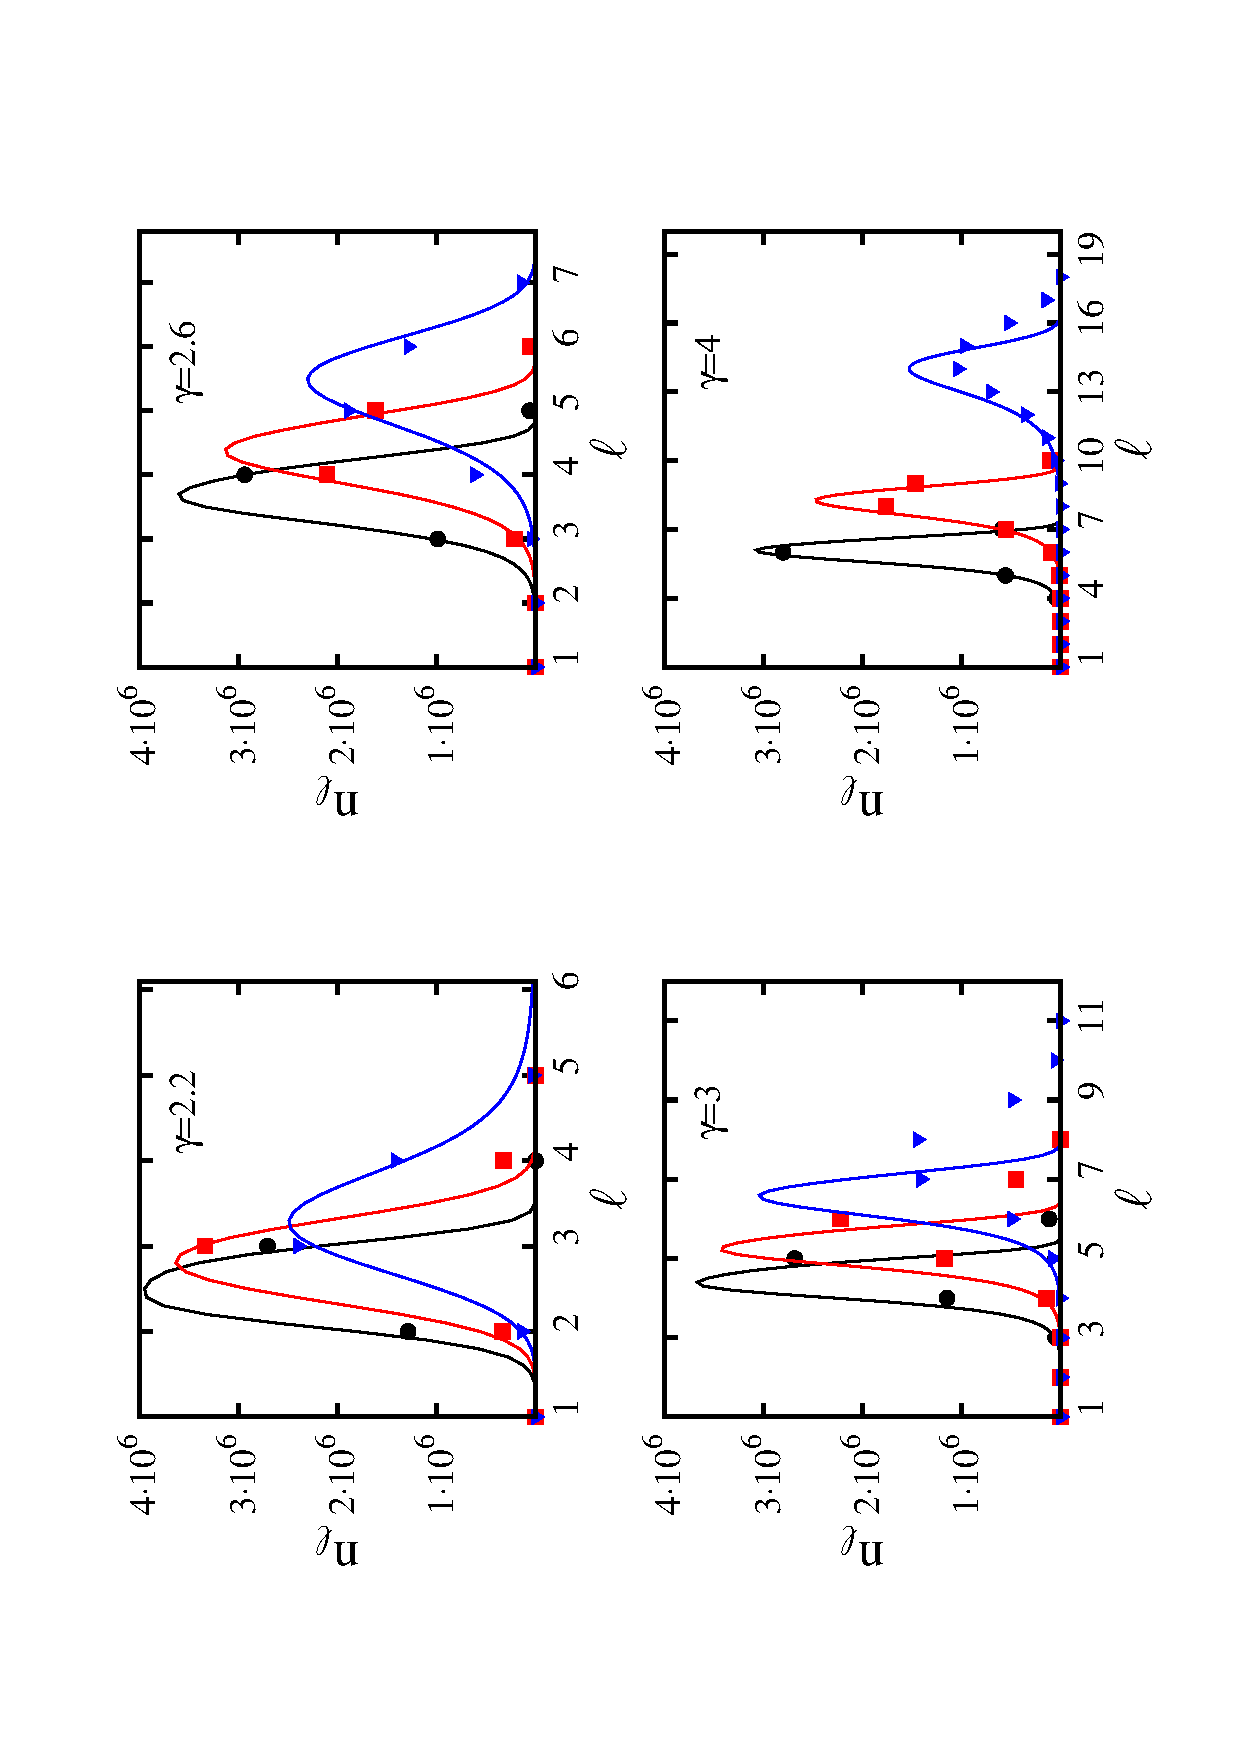
\includegraphics[angle=-90,scale=0.5]{./figures/fig2-3}
	\caption{Nombre de nœuds dans chaque couche pour différentes valeurs de $ \gamma $. Les lignes pleines sont Eq.~\eqref {eq8} et Eq.~\eqref{eq10}. Les symboles sont des simulations d'un réseau de taille $n=4\times10^6$ et une moyenne de $200$ réalisation pour chaque point. Les couleurs noir, rouge et bleu se réfèrent respectivement à $ m = 8, 4 $ et $ 2 $.}
	\label{fig2-3}
\end{figure}

Dans la Fig.~\ref{fig2-3}, nous représentons \nl en fonction de $\ell$ pour différentes valeurs de $\gamma$ et $m$. En général, un excellent accord entre la théorie et les simulations est observé. Pour $\gamma=3$, l'accord est moins bon, principalement due au fait que le réseau est encore hétérogène et que les hubs sont toujours présents, alors que nous avons supposé l'homogénéité du réseau pour calculer $\sum_{j=1}^{l} p_jn_j$ (Eq.~\eqref{eq9}).\\
Nous observons peu de différences en \nl entre la théorie et les simulations lorsque $ \gamma = 4 $ et $ m = 2 $. Ceci est causé par une augmentation relative de la proportion de cycles dans les mêmes couches. Ainsi, la structure arborescente parfaite, qui est l'hypothèse principale dans le calcul de \nl, n'est plus vraie. La figure Fig.~\ref{fig3-3} montre clairement l'augmentation relative des cycles quand $ m $ est abaissé, et $ \gamma $ augmenté.
\begin{figure}[h]
	\begin{center}
		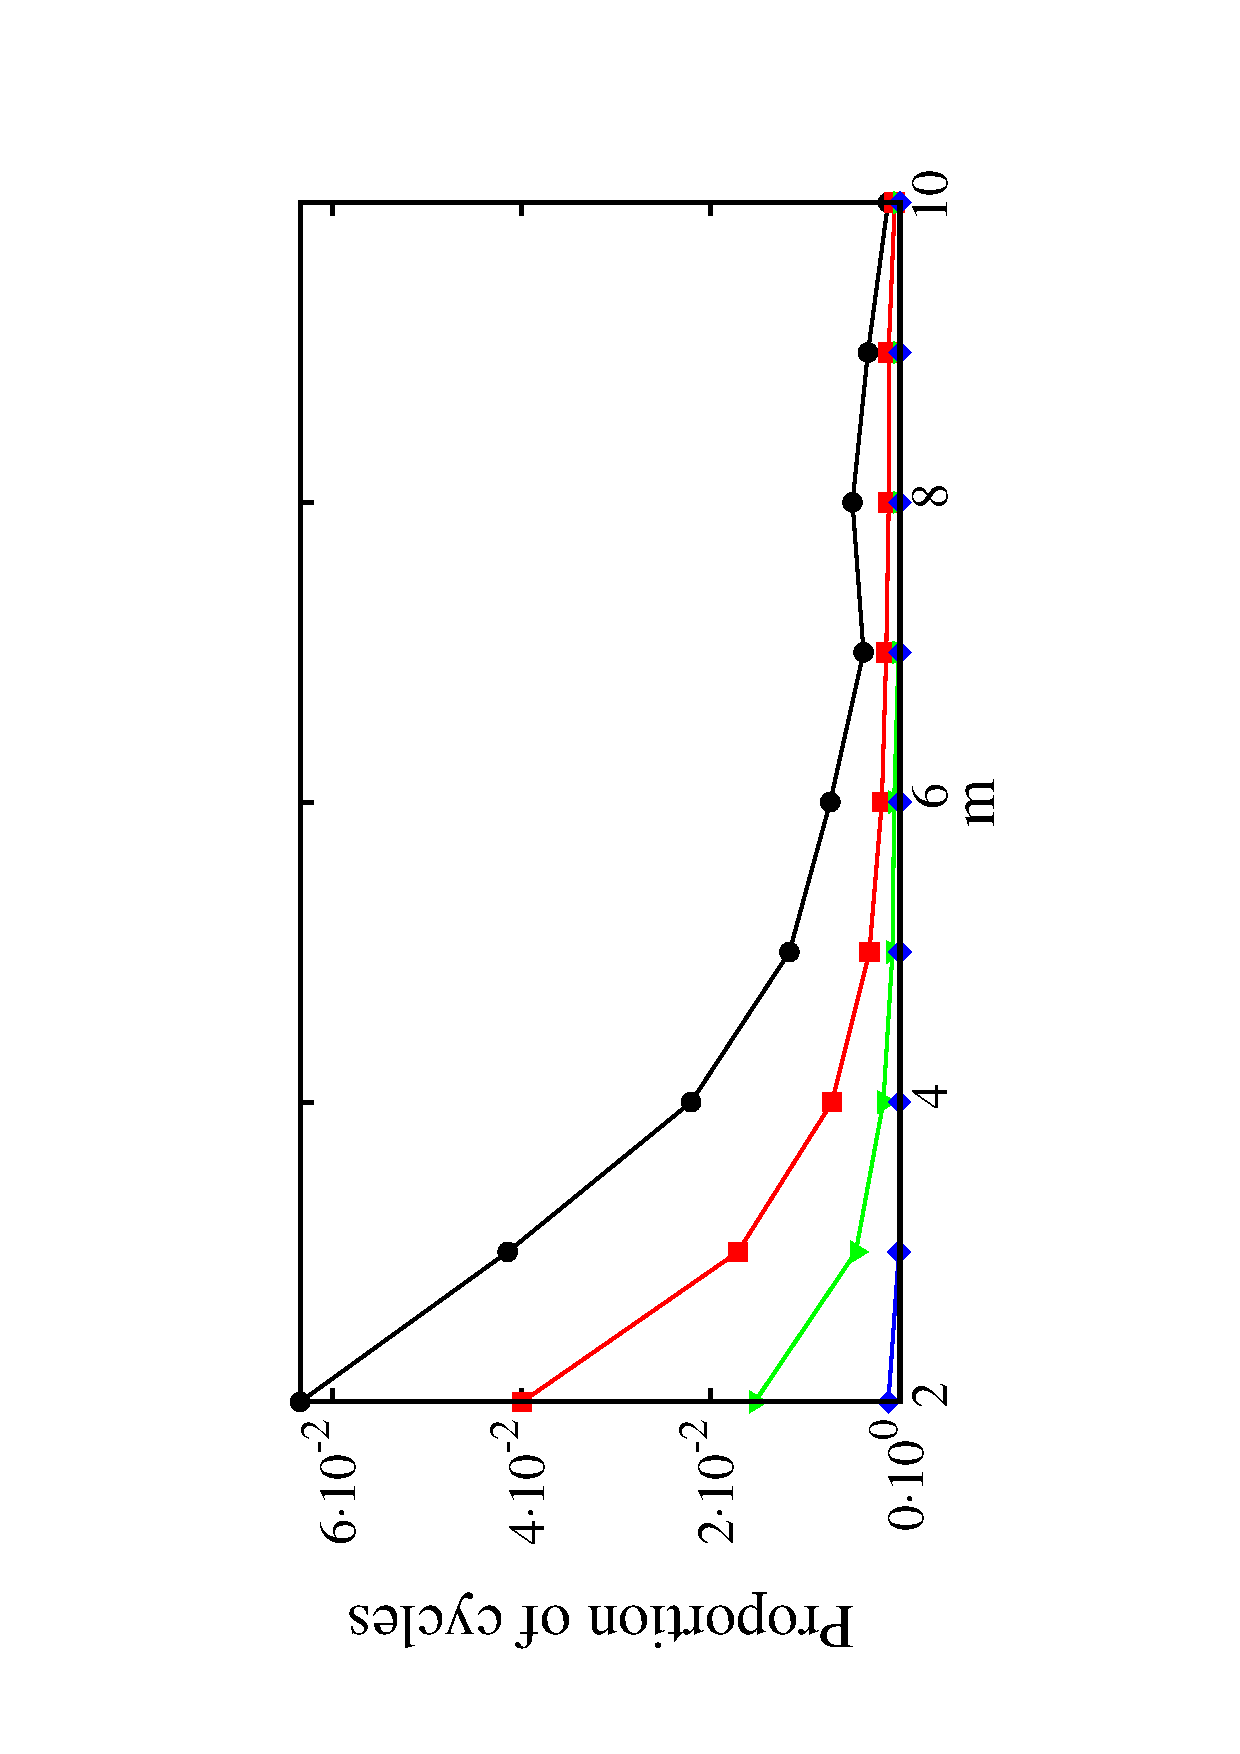
\includegraphics[angle=-90,scale=0.45]{./figures/fig3-3}
	\end{center}
	%\vspace{-10mm}
	\caption{Proportion de cycles dans les couches par rapport à $ m $. De haut en bas, $ \gamma $ est respectivement $ 4, 3, 2.6 $ et $ 2.2 $. Nombre de nœuds $ n = 4.10^6 $, le nombre de points pour chaque simulation est $200 $.}
	\label{fig3-3}
 \end{figure}
Nos résultats analytiques pour \nl sont également comparés aux réseaux du monde réel. Nous observons à partir de la figure Fig.~\ref{fig2-3} que \nl augmente et diminue de différentes manières. Les manipulations de Eq.~\eqref{eq8} et Eq.~\eqref {eq10} sont nécessaires pour extraire une information détaillée sur les queues de la distribution des nœuds. \\ Pour $n$ grand, Eq.~\eqref{eq8} pour $\ell>1$ peut être approché comme:
\begin{align}
n_{\ell}&=n\Big(e^{-\frac{\km}{n}\kappa_1^{\frac{1-\beta^{\ell-2}}{1-\beta}}}-e^{-\frac{\km}{n}\kappa_1^{\frac{1-\beta^{\ell-1}}{1-\beta}}}\Big) \nonumber \\
&\approx -n \frac{\partial \Big(e^{-\frac{\km}{n}\kappa_1^{\frac{1-\beta^{\ell-\frac{3}{2}}}{1-\beta}}} \Big) }{\partial \ell} \nonumber \\
&\approx -\frac {\km \log(\kappa_1) \log(\beta)} {1-\beta} \beta^{\ell-\frac{3}{2}} \kappa_1^{\frac{1-\beta^{\ell-\frac{3}{2}}}{1-\beta}}e^{-\frac{\km}{n}\kappa_1^{\frac{1-\beta^{\ell-\frac{3}{2}}}{1-\beta}}}, 
\label{eq11}
\end{align}
où $ \ell-\frac{3}{2} $ est utilisé à la place de $ \ell-1$ pour améliorer la différenciation avec la règle du point central. \\
Quand $\kappa_1^{\frac{1-\beta^{\ell-\frac{3}{2}}}{1-\beta}}\ll\frac{n}{\km}$,  $e^{-\frac{\km}{n}\kappa_1^{\frac{1-\beta^{\ell-\frac{3}{2}}}{1-\beta}}}\approx 1$, le terme dominant dans l'équation Eq.~\eqref{eq11} est $\kappa_1^{\frac{1-\beta^{\ell-\frac{3}{2}}}{1-\beta}}$, \nl augmente ensuite suite à une loi de puissance. Après avoir atteint son maximum à $\kappa_1^{\frac{1-\beta^{\ell-\frac{3}{2}}}{1-\beta}}=\frac{n}{\km}$, \nl diminue exponentiellement comme
$e^{-\frac{\km}{n}\kappa_1^{\frac{1-\beta^{\ell-\frac{3}{2}}}{1-\beta}}}$ quand $\kappa_1^{\frac{1-\beta^{\ell-\frac{3}{2}}}{1-\beta}}\gg\frac{n}{\km}$.\\
De la même manière, Eq.~\eqref{eq10} peut être écrit comme \nl$\approx \km \log(\kappa')\kappa'^{\ell-\frac{3}{2}}e^{-\frac{\km}{n}\kappa'^{\ell-\frac{3}{2}}}$, conduisant à un comportement de loi de puissance pour $\kappa'^{\ell-\frac{3}{2}} \ll \frac{n}{\km}$, et à une décroissance exponentielle pour $\kappa'^{\ell-\frac{3}{2}} \gg \frac{n}{\km}$.
\subsection{Comparaison avec les données réels}
La Fig.~\ref{couch-reel} représente une comparaison entre nos équations et quelques réseaux réels, nous avons choisi des réseaux réels avec différentes valeurs de $\gamma$, de $\gamma=2.13$ à $\gamma=4.831$.
% Il fait signaler que pour le réseau Hollywoodien (voir Fig.~\ref{couch-reel}.a) et Fig.~\ref{couch-reel}.b)) même que dans le réseau réel on a $\gamma=2.13$ on a prend $\gamma=2.16$ pour le cas de Kevin Bacon et $\gamma=2.12$ pour le cas de Samuel L.Jackson, mais cette confusion peut s'expliquer par les incertitudes sur la valeur de $\gamma$, ainsi que les petites changements sur la structure de réseau en relation avec le choix de nœud centrale, comme nous avons voit clairement de la Fig.~\ref{couch-reel}, la structure des couches de même réseau Hollywoodien change légèrement selon qui ayant la position au centre de réseau Bacon ou Jackson. Pour les autres réseaux réels on a prend les mêmes valeurs $\gamma$ et mêmes tailles des réseaux. 
Le réseau Digg est un réseau de réponse du site d'informations sociales, chaque nœud du réseau est un utilisateur du site Web, et chaque arête dirigée indique qu'un utilisateur a répondu à un autre. Dans le réseau Gnutella les nœuds représentent des hôtes de Gnutella, et les bords dirigés représentent des connexions entre eux. En général nos équations sont très en accord avec ces réseaux réels, ce qui donne une importance supplémentaire à notre travail concernant ce problème de couches dans les réseaux sans-échelle. 


\begin{figure}[h!]
	\centering
	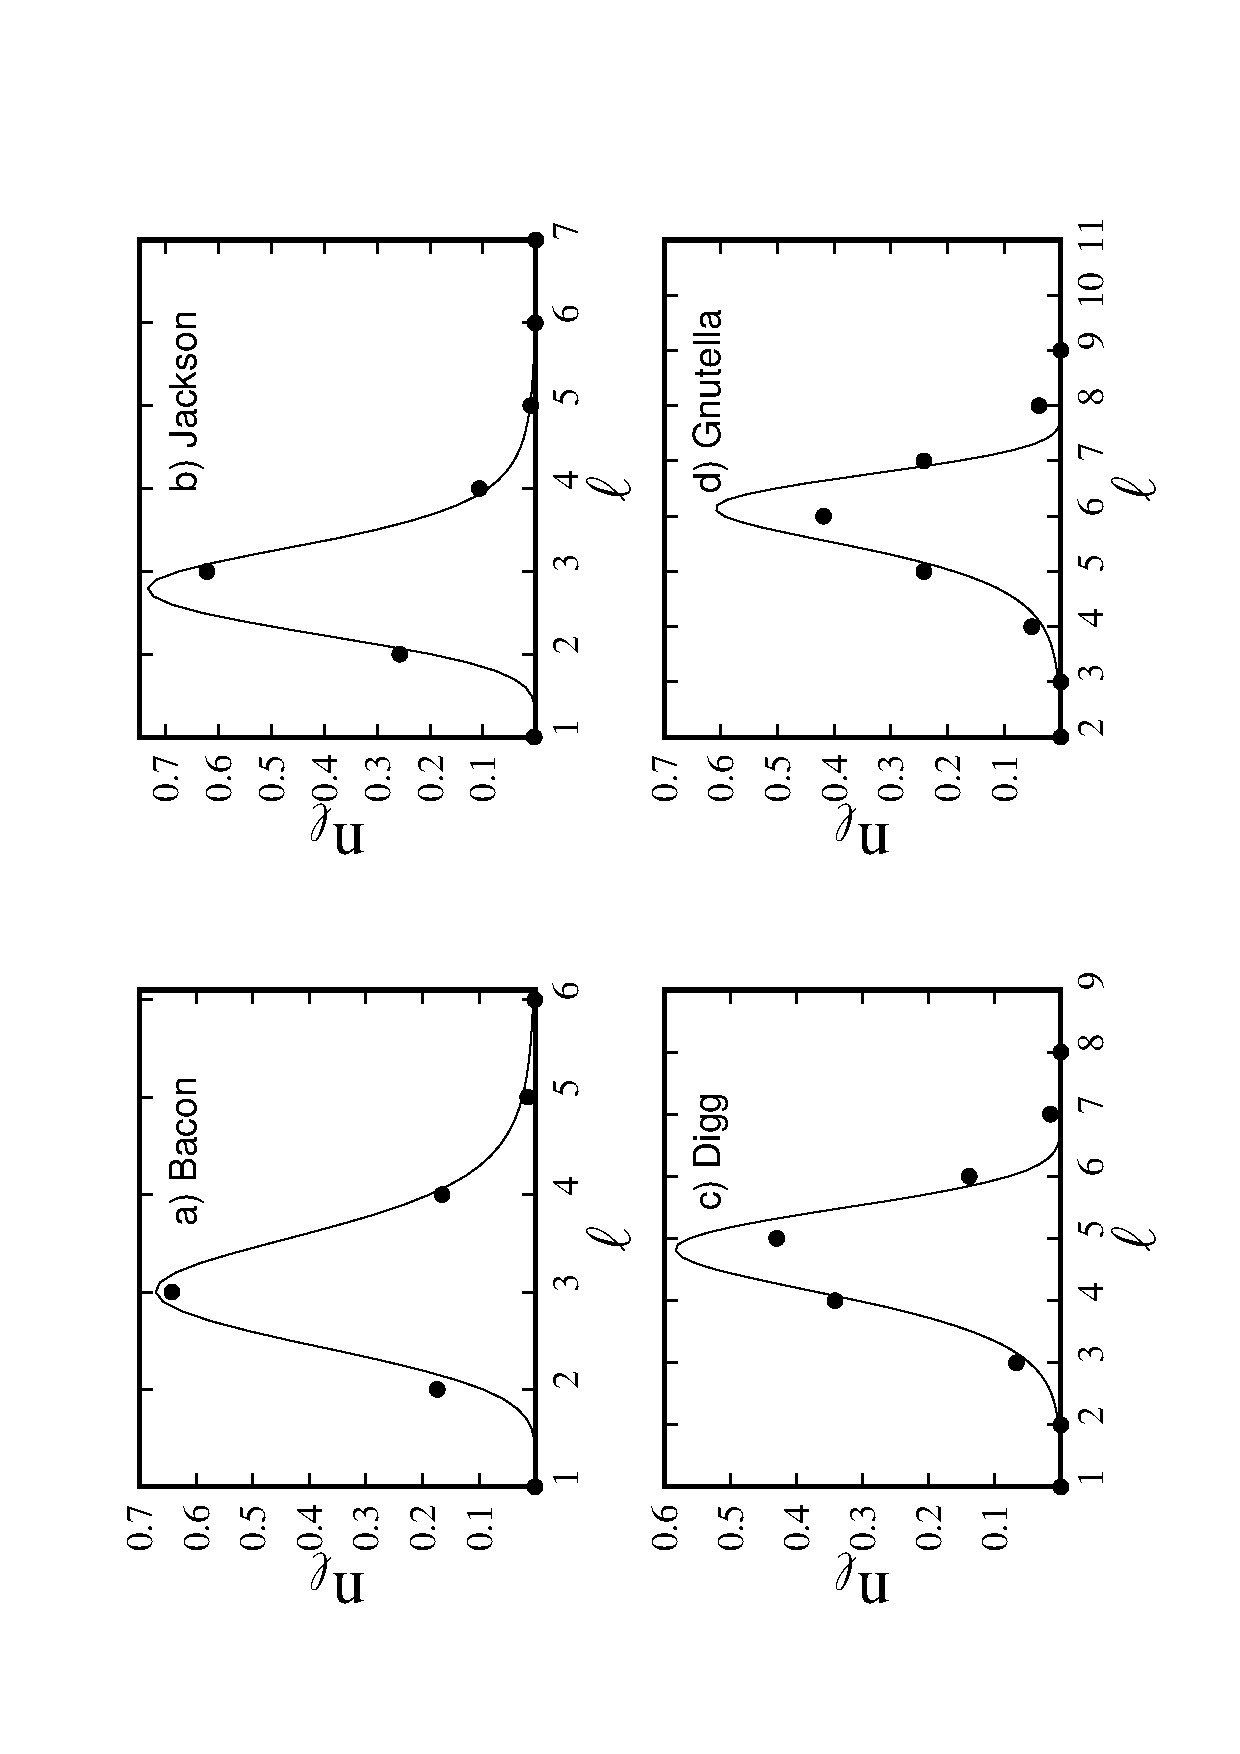
\includegraphics[scale=0.6,angle=-90]{./figures/couch-reel}
	\caption{Comparaison entre les données empiriques (cercle) de quelques réseaux réels et nos équations (ligne continue): \textbf{a)} Les cercles représentent les couches du réseau d’acteurs Hollywoodien de $2283910$ acteurs et de $\gamma=2.13$ lorsque Kevin Bacon est au centre du réseau et la ligne continue représente l'Eq.~\eqref{eq8} avec les mêmes valeurs $\gamma$ et $n$ du réseau Hollywoodien, \textbf{b)} Le même réseau Hollywoodien mais lorsque Samuel L.Jackson est au centre de réseau, \textbf{c)} Les cercles représentent les couches du réseau Digg, la ligne continue représente Eq.~\eqref{eq8} avec le même exposant $\gamma$ du réseau sociale Digg ($\gamma=2.691$) et même sa taille $n=30398$, \textbf{d)} Les cercles représentent les couches du réseau d’h{\^o}tes Gnutella, la ligne continue représente Eq.~\eqref{eq10} avec le même exposant $\gamma$ de ce réseau d’hôtes Gnutella ($\gamma=4.831$) et même sa taille $n=62586$. Tous les résultats empiriques ont été extraits des sites: "http://oracleofbacon.org/center.php" et "http://konect.uni-koblenz.de/networks/".}	
	\label{couch-reel}
\end{figure}
    
\section{Plus court chemin dans les réseaux sans-échelle non corrélés }
   \subsection{L'étude théorique}
   \label{pcc}
   Nous déduisons le PCC dans les réseaux sans-échelle non corrélés à partir de la distribution des nœuds, \nl. En fait, la forme quasi-symétrique de \nl dans la figure Fig.~\ref{fig2-3} suggère que le PCC correspond à la distance à laquelle \nl est maximal. \\ Nous commençons par le cas le plus simple $\gamma=2$. Comme déjà mentionné, il y a un maximum de deux couches dans le réseau, le PCC peut être écrit comme:
   \begin{align}
   	\textless \ell \textgreater=\frac{\km+2(n-\km)}{n},
   	\label{eq14}  
   \end{align}
qui tend vers $2$ pour un grand $n$. Cela signifie que presque tous les nœuds sont connectés en moyen au nœud de degré maximal. \\
Quand $ 2<\gamma<3 $, aucune solution pour $\frac{\partial n_{\ell}}{\partial\ell}=0$ ne peut être trouvée directement à partir de l'Eq.~\eqref{eq8}, à la place nous utilisons l'approximation donnée dans Eq.~\eqref{eq11}, où \ nl est maximal quand $\kappa_1^{\frac{1-\beta^{\textless \ell \textgreater-\frac{3}{2}}}{1-\beta}}=\frac{n}{\km}$. Après avoir remplacé $\kappa_1 $ et $K_1$ par leurs expressions correspondantes, on obtient:
\begin{align}
	\textless \ell \textgreater=\frac{\log\big(1-\frac{\log(n)-\log(\km)}{\log(n)+\frac{\gamma-1}{3-\gamma}\log(\frac{\gamma-2}{3-\gamma}m)}\big)}{\log\big(\frac{2\gamma-4}{\gamma-1}\big)}+\frac{3}{2}.
	\label{eq12}
\end{align}
pour $n$ grand, $\textless \ell \textgreater \approx -\frac{\log(\log(n))}{\log(\beta)}$.
Cette forme d'échelle est derrière la nomenclature mondiale ultra-petite \cite{Cohen-Havlin2003}, et est largement acceptée pour cette gamme de $\gamma $ \cite{Do-al2003,Cohen-al2002,Chung-Lu2002,Fox-Bellwood2014,Hofstad-al2014}.\\
Pour $\gamma\ge 3 $, le PCC peut être déduit de Eq.~\eqref{eq10} en résolvant $\frac{\partial n_{\ell}}{\partial\ell}=0$. Cela donne:
\begin{align}
	\textless \ell \textgreater=\frac{\log (n)}{\log(\kappa')}+\frac{\log(\log(\kappa'))-\log(\km)}{\log(\kappa')}+1.
	\label{eq13}
\end{align}
Si $\gamma>3$, $\kappa$ est constant (Eq.~\eqref{eq4}). Pour un grand $n$, $\textless\ell\textgreater\approx\frac{\log(n)} {\log (\kappa')}$, qui est la forme d'échelle rapportée dans de nombreux autres travaux \cite{Bollobas1985,Chung-Lu2002,Fronczak-al2004,Hofstad-al2004,Cohen-Havlin2009}, et connu comme le comportement du petit monde. \\
Quand $\gamma=3$, $\kappa$ dépend de $K$, qui dépend à son tour de $n$. Prenant $\kappa=m(\log(K)-\log(m))$ et $K=mn^{\frac{1}{\gamma-1}}$, nous trouvons pour  $n$ grand, $\textless\ell\textgreater\approx \frac{\log(n)} {\log(\log(n))} $. Ce résultat est en accord avec les travaux précédents \cite {Chung-Lu2002,Cohen-Havlin2003,Fronczak-al2004,Bollobas-Riodan2002}, et confirme le cas particulier de $ \gamma = 3 $. En effet, la présence des hubs rend les distances entre les nœuds plus petites que celles où les hubs sont absents ($\gamma>3$), en même temps les hubs ne sont pas suffisamment grands pour faire des distances ultra-petites comme $2<\gamma<3$.

\begin{figure}[h]
	\centering
	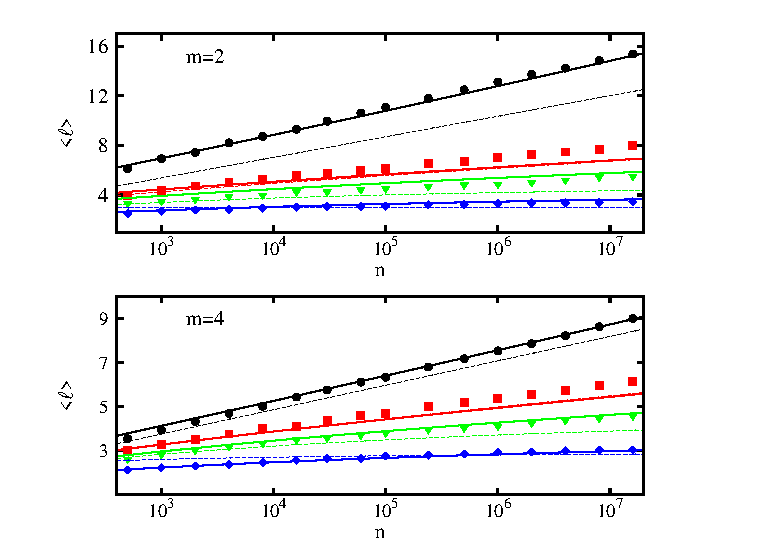
\includegraphics[scale=1.2]{./figures/fig4-3}
	\caption{La longueur moyenne du trajet en fonction du nombre de nœuds. Les valeurs de $\gamma$ de haut en bas sont respectivement $ 4, 3, 2.6 $ et $ 2.2 $. Les lignes pleines correspondent à l'équation Eq.~\eqref{eq12} et à l'équation Eq.~\eqref{eq13}. Chaque simulation est moyennée à plus de $200 $.}
	\label{fig4-3}
\end{figure}  
 
Comme nous avons signalé dans la Section.~\ref{PCC}, les travaux importants \cite{Do-al2003,Cohen-Havlin2003} dans ce sujet donnent seulement l'allure du PCC pour les grandes valeurs de $n$. L'exception est la contribution de Fronczak et  al. \cite{Fronczak-al2004} où ils ont trouvé les expressions du PCC basées sur les paramètres du réseau, leurs équations ont prédit que le PCC tend vers une valeur constante lorsque $n$ tend vers l'infini pour $2<\gamma<3$, mais celle-ci tend vers une valeur constante et cela n’est pas vrai selon les simulations numériques (voir Fig.~\ref{fig4-3}) et tous les autres résultats existant dans la littérature \cite{Do-al2003,Cohen-al2002,Chung-Lu2002,Fox-Bellwood2014,Hofstad-al2014,Cohen-Havlin2003}. De la même Fig.~\ref{fig4-3} on voit que nos résultats sont parfaitement en accord avec les simulations pour $\gamma\neq3$, pour $\gamma=3$ nos résultat sont très proches et possèdent la même allure que les simulations, ils sont également très similaires au ceux de \cite{Fronczak-al2004}.
 
\section{conclusion} 
Dans ce chapitre, nous avons étudié en détail certains aspects fondamentaux des réseaux sans-échelle non corrélés. Avec des étapes et des hypothèses simples, nous avons obtenu des expressions explicites, en fonction de l'exposant de degré $\gamma$, pour le nombre des nœuds à une distance donnée d'un nœud arbitraire, \nl\nolinebreak, ainsi qu'une description précise de la formule de distribution \nolinebreak. En plus, nous avons montré que \nl augmente suivant la loi de puissance pour les quelques premières couches, et après avoir atteint un maximum il diminue exponentiellement dans les dernières couches.
Profitant de la formule de distribution \nl, nous avons pu déduire l'expression explicite du PCC. Les expressions obtenues reproduisent les formes de mise à l'échelle connues pour différentes plages de $\gamma$. Autrement dit, le monde ultra-petit pour $2<\gamma<3$, et le petit monde pour $\gamma\ge 3$. Nos résultats théoriques concordent très bien avec les simulations, sauf dans le cas de $\gamma=3$, où nous avons observé la même forme, comme pour les autres valeurs de $\gamma$, dans les queues de \nl, mais avec une notable différence dans la position du maximum. Cette différence n'affecte pas la forme de mise à l'échelle du PCC pour cette valeur de $\gamma$.